\documentclass{thesisclass}
% Based on thesisclass.cls of Timo Rohrberg, 2009
% ----------------------------------------------------------------
% Thesis - Main document
% ----------------------------------------------------------------


%% -------------------------------
%% |  Information for PDF file   |
%% -------------------------------
\hypersetup{
 pdfauthor={Daniel Lipp},
 pdftitle={EAs for Partition},
 pdfsubject={?},
 pdfkeywords={?}
}


%% ---------------------------------
%% | Information about the thesis  |
%% ---------------------------------

\newcommand{\myname}{Lipp Daniel}
\newcommand{\mytitle}{Theoretical and empirical runtime analysis of evolutionary algorithms for the partition problem}
\newcommand{\myinstitute}{Chair of algorithms for intelligent systems}

\newcommand{\reviewerone}{?}
\newcommand{\reviewertwo}{?}
\newcommand{\advisor}{Prof.\ Dr.\ Dirk Sudholdt}
\newcommand{\advisortwo}{?}

\newcommand{\timestart}{14th May 2023}
\newcommand{\timeend}{14th August 2023}


%% ---------------------------------
%% | Commands                      |
%% ---------------------------------

\newtheorem{definition}{Definition} \numberwithin{definition}{chapter}
\newtheorem{theorem}[definition]{Theorem}
\newtheorem{lemma}[definition]{Lemma}
\newtheorem{corollary}[definition]{Corollary}
\newtheorem{conjecture}[definition]{Conjecture}


%% --------------------------------
%% | Settings for word separation |
%% --------------------------------
% Help for separation:
% In german package the following hints are additionally available:
% "- = Additional separation
% "| = Suppress ligation and possible separation (e.g. Schaf"|fell)
% "~ = Hyphenation without separation (e.g. bergauf und "~ab)
% "= = Hyphenation with separation before and after
% "" = Separation without a hyphenation (e.g. und/""oder)

% Describe separation hints here:
\hyphenation{
% Pro-to-koll-in-stan-zen
% Ma-na-ge-ment  Netz-werk-ele-men-ten
% Netz-werk Netz-werk-re-ser-vie-rung
% Netz-werk-adap-ter Fein-ju-stier-ung
% Da-ten-strom-spe-zi-fi-ka-tion Pa-ket-rumpf
% Kon-troll-in-stanz
}


%% ------------------------
%% |    Including files   |
%% ------------------------
% Only files listed here will be included!
% Userful command for partially translating the document (for bug-fixing e.g.)
\includeonly{
titlepage,
introduction,
preliminaries,
content,
conclusion,
appendix
}


%%%%%%%%%%%%%%%%%%%%%%%%%%%%%%%%%
%% Here, main documents begins %%
%%%%%%%%%%%%%%%%%%%%%%%%%%%%%%%%%
\begin{document}

% Remove the following line for German text
\selectlanguage{english}

\frontmatter
\pagenumbering{roman}
%% titlepage.tex
%%

\begin{titlepage}

  \iffalse
  \begin{textblock}{10}[0,0](4,2.5)
		
\includegraphics[]{logos/UPLogo.pdf}
	\end{textblock}
        \begin{textblock}{10}[0,0](14.5,2.45)
          
\includegraphics[]{logos/UPLogo.pdf}
	\end{textblock}
\fi

        \changefont{phv}{m}{n}	% helvetica	
	\vspace*{3.75cm}
	\begin{center}
		\Huge{\mytitle}
		\vspace*{2.25cm}\\
		\Large{
			\iflanguage{english}{Bachelor Thesis of}			
												  {Masterarbeit\\von}
		}\\
		\vspace*{1cm}
		\huge{\myname}\\
		\vspace*{1cm}
		\Large{
			\iflanguage{english}{At the Department of Informatics and Mathematics}			
													{An der Fakult\"at f\"ur Informatik und Mathematik}
			\\
			\myinstitute\\
                      }
	\end{center}
        \begin{center}
        
\includegraphics[]{logos/UPLogo.pdf}
      \end{center}

	\vspace*{1cm}
                      

        \Large{
\begin{center}
\begin{tabular}[ht]{l c l}
  % Gutachter sind die Professoren, die die Arbeit bewerten. 
  \iflanguage{english}{Reviewers}{Erstgutachter}: & \hfill & \reviewerone\\
  \iflanguage{english}{}{Zweitgutachter:} & \hfill & \reviewertwo\\
  \iflanguage{english}{Advisors}{Betreuende Mitarbeiter}: & \hfill & \advisor\\
  \iflanguage{english}{}{} & \hfill & \advisortwo\\
  % Betreuende Mitarbeiter wenn nicht vorhanden ggf. weglassen. 
\end{tabular}
\end{center}
}


\vspace{2cm}
\begin{center}
\large{\iflanguage{english}{Time Period}{Bearbeitungszeit}: \ \timestart{} \ -- \ \timeend}
\end{center}

\end{titlepage}

\blankpage

%% -------------------------------
%% |   Statement of Authorship   |
%% -------------------------------

\thispagestyle{plain}

\vspace*{\fill}

\centerline{\textbf{Statement of Authorship}}

\vspace{0.25cm}

I hereby declare that this document has been composed by myself and describes my own work, unless otherwise acknowledged in the text.

\vspace{2.5cm}

\hspace{0.25cm} Passau, \today

\vspace{2cm}

\blankpage

%% -------------------
%% |   Abstract      |
%% -------------------

\thispagestyle{plain}

\begin{addmargin}{0.5cm}

\centerline{\textbf{Abstract}}

A short summary of what is going on here.

\vskip 2cm

\centerline{\textbf{Deutsche Zusammenfassung}}

Kurze Inhaltsangabe auf deutsch.

\end{addmargin}

\blankpage

%% -------------------
%% |   Directories   |
%% -------------------

\tableofcontents
\blankpage

%% -----------------
%% |   Main part   |
%% -----------------

\mainmatter
\pagenumbering{arabic}
%% introduction.tex
%%

%% ==============================
\chapter{Introduction}\label{ch:introduction}
%% ==============================

% This chapter should contain
% \begin{enumerate}
%   \item A short description of the thesis topic and its background.
%   \item An overview of related work in this field.
%   \item Contributions of the thesis.
%   \item Outline of the thesis.
% \end{enumerate}

The question of $P=NP$ is still unanswered to this day and solving $NP$-hard problems for every instance still requires exponential time.
To avoid the exponential running time on $NP$-hard optimisation problems one might use approximation algorithms.
Those algorithms do not always return the best possible solution but only a solution with a guaranteed solution quality.
For a minimisation problem a (1+0.5)-approximation algorithm will always return a solution that has at most 1.5 times the optimal value.
An example of an $NP$-hard optimisation problem is PARTITION.\ 
An instance of this problem is a multiset of $n$ positive numbers $\{w_1,\dots,w_n\}$ which has to be divided in two subsets with sums that are as close as possible.
So a solution of PARTITION is a subset of $I\subset \{1,\dots,n\}$ which splits the multiset into two subsets.
The quality of the solution then is $\max\{\sum_{i\in I}w_i, \sum_{i\notin I}w_i\}$.
PARTITION is one of the easiest $NP$-hard problems and has even been dubbed the easiest $NP$-hard problem~\cite{hayes2002computing}.
There are multiple algorithms specifically designed for PARTITION.\ 
Some of them return approximations and others always return the best solution.
The exact algorithms have a runtime exponential in the input size due to the $NP$-hardness.
Problem specific approximation algorithms are mostly deterministic such as the greedy method, the KK-algorithm or the FPTAS for the subsetsum problem which can be used for partition as well.
Another class of non-deterministic algorithms are the so-called Evolutionary Algorithms which mimic the behaviour of evolution.
Those algorithms start with a random population of solutions which are then changed with random steps.
If the solution is good enough it survives and replaces one of the worst individuals in the population.
The EA continues to generate new offspring in an endless loop.
In practice the algorithm is given stopping conditions such as reaching a number of iterations or a specific solution quality.
This is the principle of an anytime algorithm which can be terminated at anytime and output a valid solution.
The longer the waiting time the better the solution might get.
The main usage of EA lies in problems without a problem specific algorithms as these mostly outperform the EAs.
To better understand their behaviour analysing them on well researched problems might still be beneficial to learn more about this class of algorithms.
This thesis researches the runtime of basic EAs such as (1+1) EA and variations of the RLS.\ 
The first part is a theoretical analysis with a main focus of lowering bounds that were previously shown.
Additionally there are new results for other algorithm variants and also a lemma on different type of inputs.
The remainder of this thesis is an empirical analysis of multiple base algorithms with different parameter setting on different kinds of inputs.
Here not only the (1+1) EA with different mutation rate and variants of the RLS with different parameter values are researched but also a heavy tailed mutation operator.
Apart from typical distributions such as the uniform, geometric and binomial distribution there are also results for problem specific instances such as an input where one values is as large as all other values combined.
In the end the empirical results are condensed into a personal suggestion which algorithm should best be chosen to solve the problem, depending on the input but also in general.


%% preliminaries.tex
%%

%% ==============
\chapter{Preliminaries}
\label{ch:preliminaries}
%% ==============

This chapter should provide the foundations of the thesis.
%% content.tex
%%

%% ==============
\chapter{Content Chapters}
\label{ch:Content1}
%% ==============

% The content chapters of your thesis should of course be renamed. How many chapters you need to write depends on your thesis and cannot be said in general.

%  Always reference figures, tables etc. To give a few simple examples, this section contains Algorithm \ref{theorem:doof}, Table \ref{tbl:randomnumbers}, Figure \ref{fig:somegraph}, and Theorem \ref{theorem:doof}. To give an example citation we recommend the book of Garey and Johnson \cite{gj-ci-79}.

% \begin{algorithm}[bt]
% \caption{\textsc{Dijkstra}}\label{alg:dijkstra}

% % Some settings
% \DontPrintSemicolon %dontprintsemicolon
% \SetFuncSty{textsc}
% \SetKwFor{ForAll}{forall}{do}

% % Declaration of data containers and functions
% \SetKwData{Q}{Q}
% \SetKwData{dist}{d}
% \SetKwData{pred}{pred}
% \SetKwFunction{queueDeleteMin}{deleteMin}
% \SetKwFunction{queueInsert}{insert}
% \SetKwFunction{queueDecreaseKey}{decreaseKey}
% \SetKwFunction{queueContains}{contains}

% % Algorithm interface
% \KwIn{Graph $G = (V,E,\omega)$, source node $s$}
% \KwData{Priority queue \Q}
% \KwOut{Distances \dist{$v$} for all $v \in V$, shortest-path tree of $s$ given by \pred{$\cdot$}}

% % The algorithm
% \BlankLine
% \tcp{Initialization}
% \ForAll{$v \in V$}{$\dist{v} \leftarrow \infty$ \; $\pred{v} \leftarrow \texttt{null}$}
% \Q.\queueInsert{$s,0$}\; $\dist{s} \leftarrow 0$ \;
% \BlankLine
% \tcp{Main loop}
% \While{\Q is not empty}
% {
%   $u \leftarrow$ \Q.\queueDeleteMin{} \;
%   \ForAll{ $(u,v) \in E$ }
%   {
%     \If{$\dist{u} + \omega(u,v) < \dist{v}$}
%     {
%       $\dist{v} \leftarrow \dist{u} + \omega(u,v)$ \;
%       $\pred{v} \leftarrow u$ \;
%       \uIf{\Q.\queueContains{v}}
%       {
%         \Q.\queueDecreaseKey{$v, \dist{v}$}
%       }
%       \Else
%       {
%         \Q.\queueInsert{$v, \dist{v}$}
%       }
%     }
%   }
% }
% \end{algorithm}

% \begin{table} [bt]
% \centering
% \caption{Some strange numbers.}
% \begin{tabular}{rr}
% \toprule
% First column & Second column \\
% \midrule
% 3\,109\,218\,136 & 3\,208\,415\,108 \\
% 2\,231\,385\,058 & 1\,959\,477\,358 \\
% 1\,287\,719\,872 & 1\,317\,165\,206 \\
% 2\,516\,844\,936 & 2\,630\,583\,944 \\
% 1\,569\,466\,774 & 1\,636\,507\,220 \\
% 1\,032\,627\,816 &    991\,322\,491 \\
% \bottomrule
% \end{tabular}
% \label{tbl:randomnumbers}
% \end{table}

% \begin{figure} [bt]
%   \centering
%   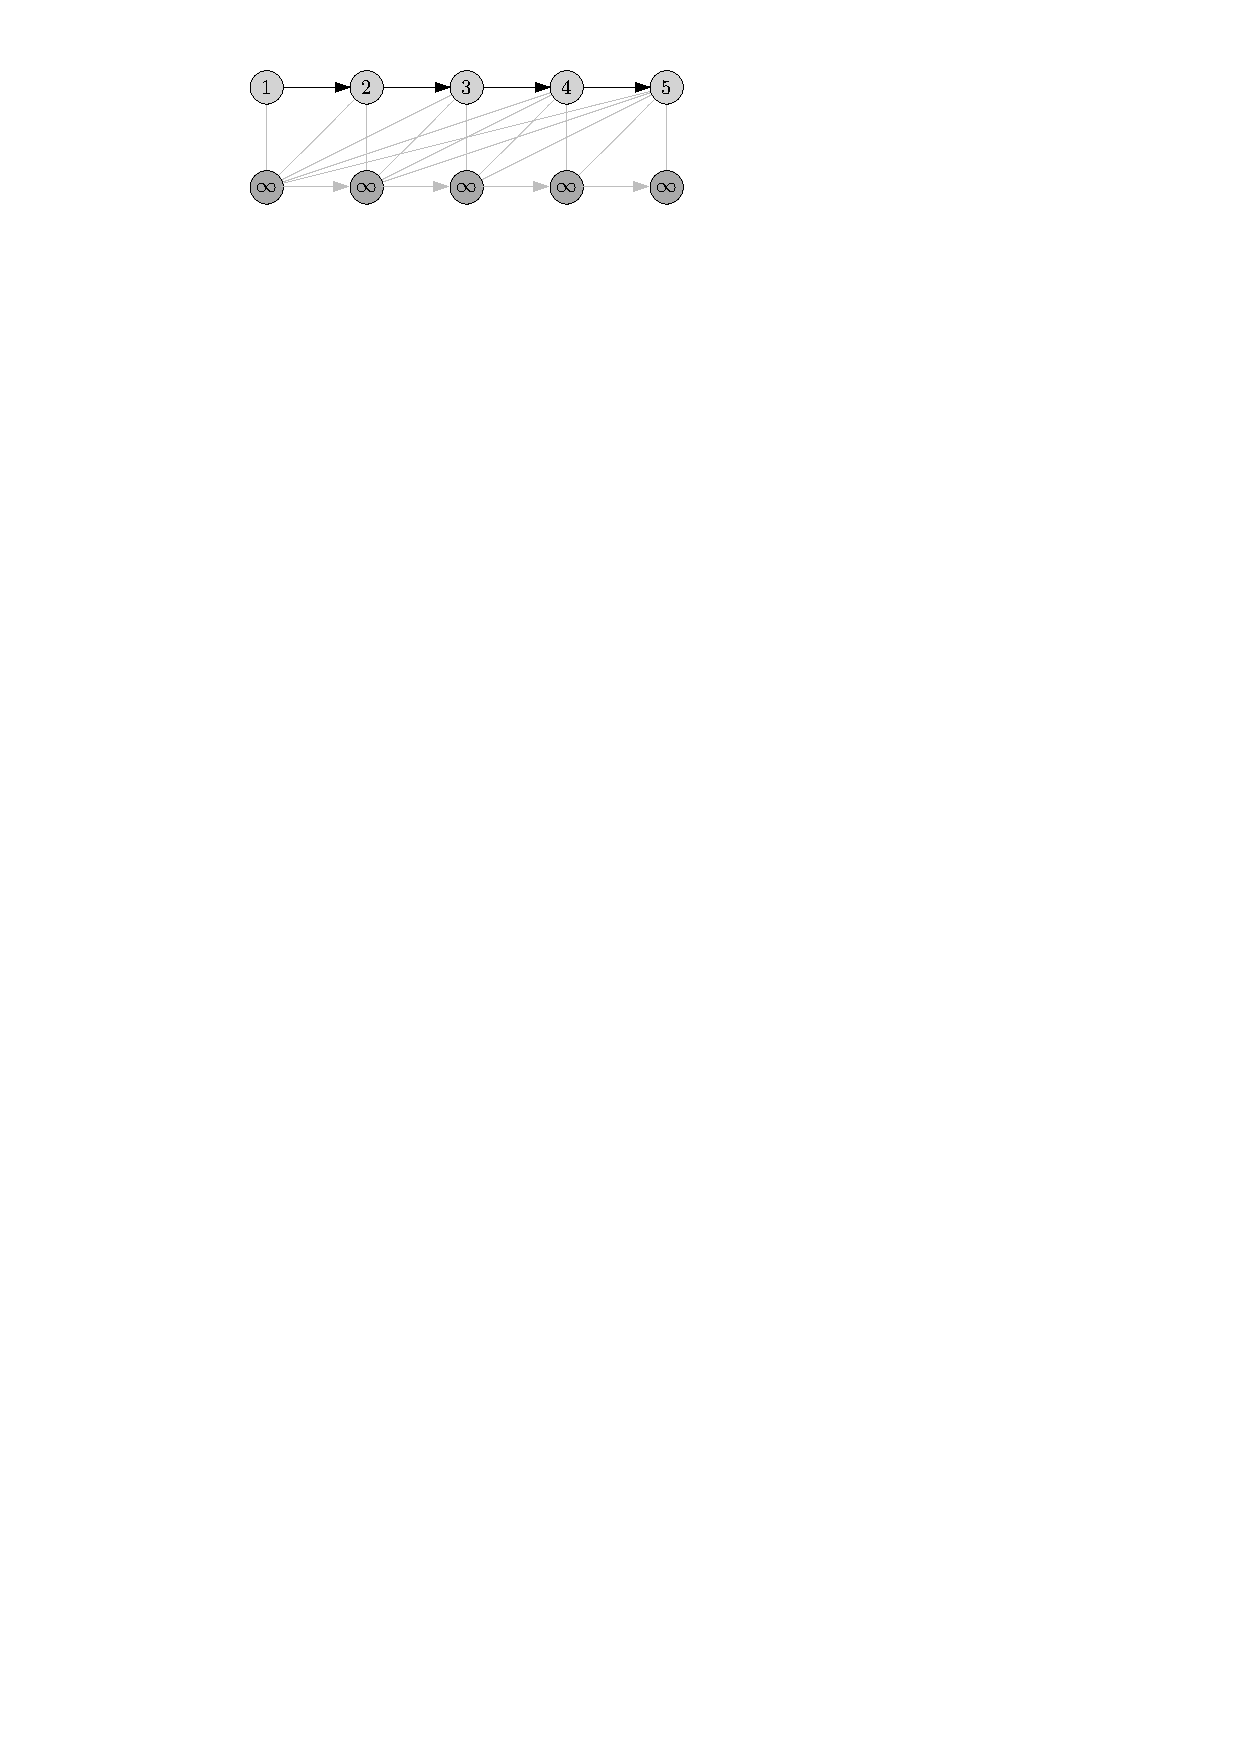
\includegraphics{figures/somegraph}
%   \caption{A funny graph.}
%   \label{fig:somegraph}
% \end{figure}
%% conclusion.tex
%%

%% ==================
\chapter{Conclusion}
\label{ch:conclusion}
%% ==================

There is no clear best algorithm for every input for PARTITION and not even a best parameter for every algorithm.
For inputs that are comparable to a linear function/OneMax for all base algorithms the parameter with the lowest mutation rate has the best runtime.
Other instances like the worst case input of C. Witt on the other hand require much higher mutation rates for the optimal performance.
Inputs generated from a powerlaw distribution showed that the optimal parameter for every algorithm is not even fixed within a specific distribution.
For inputs drawn from \textasciitilde$D^{2.75}_{50000}$ the higher mutation rates reached an optimum faster than the lower mutation rate for every algorithm variant.
If the input was drawn from \textasciitilde$D^{1.25}_{50000}$ then the fastest mutation rates for the (1+1) EA on \textasciitilde$D^{2.75}_{50000}$ distributed inputs then instead became the slowest.\newline
So almost no general advice is possible, but a few points still hold for every input type.
The first one is the RLS being most likely to be stuck in a local optimum especially for the smaller input size.
Even if a variant of the RLS is the fastet for the bigger input sizes it is most likely to be stuck in a local optimum for $n\le100$ for most input types.
So if the input size $n\le100$ choosing the (1+1) EA or $pmut$ mutation operator is a better choice.
Another noticeable relation is that inputs that require higher mutation rates are generally easy to solve and are also solved very fast by the lower mutation rates.
A lower number of iterations also does not imply a shorter runtime in every case.
If the mutation rate $1/n$ needs only a few iterations more than $100/n$ it will still be much faster since one iteration is much shorter.
The lower mutation rates are therefore generally a better choice as they will need less time in most cases and are still rather fast if they are not the fastest.
Only if the algorithm is trapped due to its low mutation rate a higher mutation rate makes a huge difference.\newline
Another point is that the Evolutionary Algorithms perform better for larger input sizes as there are more perfect partitions.
The more perfect partition an input has, the easier it is to find one.
For the lower values of $n$ the algorithm sometimes needed 20,000 iterations on average if they managed to find a perfect partition and even longer otherwise.
A runtime of \(100,000\approx2^{14,29}\ge 2^{n-6}\ge2^{n/2}\) is exponential in the size of the input.
So for smaller values choosing other approximation algorithms or even exact algorithms will probably lead to better a better runtime.
For higher values of $n$ on easier inputs they might be efficient as well or in some cases even better.\newline
The last common relation is the less small values especially close to 1 an input has the better flipping 2 or 4 bits in a step becomes.
This was only shown for the binomial distributed inputs but on inputs from \textasciitilde$U(10^4,5\cdot 10^5)$ the results were mostly the same.
To make the thesis shorter this was not listed in the corresponding section.

\begin{table}[t]
      \caption{Best algorithms variants for all evaluated input types}
      \begin{tabular}{c|ccc|ccc|ccc}\label{table:BestAlgoVariantsTable}
                                                   &
            \multicolumn{3}{c|}{RLS variants}      &
            \multicolumn{3}{c|}{(1+1) EA variants} &
            \multicolumn{3}{c}{$pmut$ variants}                                                                                      \\
                                                   & 1st      & 2nd      & 3rd      & 1st     & 2nd    & 3rd    & 1st  & 2nd  & 3rd  \\\hline
            binomial                               & \RLSN[2] & \RLSN[4] & \RLSR[2] & 3$/n$   & 4$/n$  & 2$/n$  & 2.0  & 2.25 & 2.5  \\
            geometric                              & \RLSR[2] & \RLSR[3] & \RLSR[4] & 2$/n$   & 1$/n$  & 3$/n$  & 3.25 & 3.0  & 2.75 \\
            uniform                                & \RLSN[2] & \RLSR[3] & \RLSR[4] & 4$/n$   & 3$/n$  & 2$/n$  & 2.0  & 2.25 & 2.75 \\
            polwerlaw                              & \RLSR[4] & \RLSN[3] & \RLSR[3] & 4$/n$   & 3$/n$  & 5$/n$  & 1.5  & 1.75 & 1.25 \\
            linear function                        & RLS      & \RLSR[2] & \RLSR[3] & 1$/n$   & 2$/n$  & 3$/n$  & 3.5  & 3.25 & 3.0  \\
            worst case                             & \RLSN[4] & \RLSR[4] & \RLSN[3] & 100$/n$ & 50$/n$ & 10$/n$ & 1.25 & 1.5  & 1.75 \\
            combined                               & RLS      & \RLSR[2] & \RLSR[3] & 1$/n$   & 2$/n$  & 3$/n$  & 3.25 & 3.0  & 2.75 \\
      \end{tabular}
\end{table}

Now to round this paper up there are two tables that summarise the previous results.
For each input type and each algorithm the best three variants are listed in Table~\ref{table:BestAlgoVariantsTable} ordered by their average runtime.
This implies a general tendency of better algorithms but is not necessarily a complete insight as the best parameter and algorithm changes depending on $n$.
Table~\ref{table:BestAlgoVariantTable} list my personal preference based on the previous results depending on the distribution and size of the input.
There is no clear overall winner but if one algorithm must be chosen for any input then choosing $pmut_{2.25}$ should be a good option.
For binomial distributed inputs the \RLSN[2] and the \RLSN[4] are the fastest RLS variants but for the OneMax equivalent they need about \(\Theta(\frac{n^k}{k!})\) iterations on average and expectation.
The runtime of the other RLS variants is also too unstable.
So the RLS versions are too much dependent on the input and should not be chosen in every case, especially if the input size is small.
For the best (1+1) EA variants this does not to that extend as the mutation rate $3/n$ is under the top 3 for every input type except the worst case input.
Yet on the OneMax input and the worst case input the (1+1) EA with mutation rate $3/n$ does not reach the optimal solution in all runs in at most $10n\ln{n}$ steps.
$pmut_{2.25}$ is not always one of the best three $pmut$ variants but is also never one of the worst and for the bigger input sizes it also reaches the optimal solution for almost any input in $10n\ln{n}$ steps except for 2/10,000 runs for the Worst Case input of C. Witt.
So if only one algorithm for every input must be chosen, then $pmut_{2.25}$ should be one of the best options.

\begin{table}[h]
      \caption{Suggestions for the fastest algorithm on each input depending on the input size (the (1+1) EA is listed as EA to make the table shorter)}
      % \begin{tabular}{cccccccccc}\label{table:BestAlgoVariantTable}
      \begin{tabular}{m{2.5cm}m{1cm}m{1cm}m{0.5cm}m{0.5cm}m{0.5cm}m{0.5cm}m{0.5cm}m{0.5cm}m{1cm}m{1cm}}\label{table:BestAlgoVariantTable}
            input size $n$  & \multicolumn{2}{|c}{$100$}                          & \multicolumn{2}{c}{$500$}
                            & \multicolumn{2}{c}{$1000$}                          & \multicolumn{2}{c}{$5000$}
                            & \multicolumn{2}{c}{$50,000$}                                                                                         \\
            \hline
            geometric       & \multicolumn{5}{|c|}{EA $_{2/n}$}                   & \multicolumn{4}{c|}{$pmut_{3.25}$} & RLS                       \\
            \hline
            binomial        & \multicolumn{3}{|c|}{EA $_{3/n}$}                   &
            \multicolumn{7}{c}{\multirow{2}{*}{\RLSN[2]}}                                                                                          \\
            uniform         & \multicolumn{3}{|c|}{EA $_{4/n}$}                   & \multicolumn{7}{c}{}                                           \\
            \hline
            powerlaw        & \multicolumn{10}{|c}{$pmut_{1.5}$ or $pmut_{1.75}$}                                                                  \\
            \hline
            linear function & \multicolumn{10}{|c}{RLS}                                                                                            \\
            \hline
            worst case      & \multicolumn{10}{|c}{$pmut_{1.25}$}                                                                                  \\
            \hline
            combined        & \multicolumn{1}{|c|}{EA $_{2/n}$}                   & \multicolumn{6}{c|}{$pmut_{3.25}$} & \multicolumn{3}{c}{RLS}   \\
                            &                                                     &                                    &
                            &                                                     &                                    &
                            &                                                     &                                    &                         & \\
      \end{tabular}
\end{table}



%% --------------------
%% |   Bibliography   |
%% --------------------

\cleardoublepage
\phantomsection
\addcontentsline{toc}{chapter}{\bibname}

\iflanguage{english}
{\bibliographystyle{alpha}}
{\bibliographystyle{babalpha-fl}} % german style

\bibliography{references}


%% ----------------
%% |   Appendix   |
%% ----------------

\cleardoublepage
%% appendix.tex
%%

%% ==============================
%\chapter{Appendix}
%\label{ch:Appendix}
%% ==============================

\appendix

\iflanguage{english}
{\addchap{Appendix}}	% english style
{\addchap{Anhang}}	% german style


\section{Appendix Section 1}
\label{appendix1}

\begin{figure} [ht]
  \centering
   ein Bild
  \caption{A figure}
  \label{fig:BPMNBeispiela}
\end{figure}




\end{document}
